\documentclass[10.5pt,a4paper]{article}
\usepackage{iftex}
\ifPDFTeX
  \usepackage[T1]{fontenc}
  \usepackage[utf8]{inputenc}
  \usepackage{lmodern}
\else
  \usepackage{fontspec}
\fi
\usepackage[margin=2cm,top=1.8cm,bottom=1.7cm]{geometry}
\usepackage{microtype}
\usepackage{array}
\usepackage{booktabs}
\usepackage{tabularx}
\usepackage{enumitem}
\usepackage{xcolor}
\usepackage{tikz}
\usetikzlibrary{arrows.meta,positioning,calc}
\usepackage[hidelinks]{hyperref}

\pagestyle{empty}
\setlength{\parindent}{0pt}
\setlength{\parskip}{4pt}
\setlength{\emergencystretch}{3em}
\setlist{nosep,leftmargin=1.3em,topsep=2pt}
\newcolumntype{Y}{>{\raggedright\arraybackslash}X}
\newcolumntype{P}[1]{>{\raggedright\arraybackslash}p{#1}}
\renewcommand{\arraystretch}{1.12}
\newcommand{\head}[1]{\vspace{5pt}{\large\bfseries #1}\par\vspace{1pt}}

\tikzset{
  >={Stealth[length=2mm,width=1.5mm]},
  box/.style={draw, rounded corners=2pt, align=center, inner sep=3pt,
    minimum height=9mm, fill=white, font=\footnotesize},
  gbox/.style={box, fill=black!7},
  hbox/.style={box, fill=black!16},
}

\begin{document}

{\LARGE\bfseries Semantic Trust Layer (STL): Prototype Plan}\par
\vspace{4pt}
\begin{tabular}{@{}ll@{}}
\textbf{To:} & Maj. Babar, Project Supervisor \\
\textbf{From:} & Muhammad Abdul Ghani Qureshi (F23607005) \\
\textbf{Group:} & Muhammad Usman Nasir (F23607004) and Raja Mahad Ali (F23607035) \\
\textbf{Date:} & 5 November 2026 \\
\end{tabular}

\vspace{4pt}
Sir, this note explains what our group wants to build in the first stage of our project, so that we agree on it before implementation starts. The proposal and slides show the full vision. This note covers the prototype.

\head{1. What we want to build}
We want to build an AI semantic layer. It sits in the path of incoming data and decides whether each item should be flagged. The main point is that it judges data by its meaning, using AI agents. Keyword lists and fixed rules do not make the decision.

Two AI agents work at the same time on the same incoming data:

\begin{itemize}
  \item \textbf{Application Agent} reads the content: an email, a message, a link, a QR code destination or the text of a file. It asks what the content is saying and what it wants the reader to do.
  \item \textbf{Network Agent} reads how the data travels: flows, timing, sizes, DNS and TLS metadata. It asks how the sender or connection is behaving. It does not need the content, so it still works on encrypted traffic.
  \item \textbf{Coordinator} joins both findings, gives one verdict (allow, warn, flag or block) and states the reason in plain words.
\end{itemize}

\begin{center}
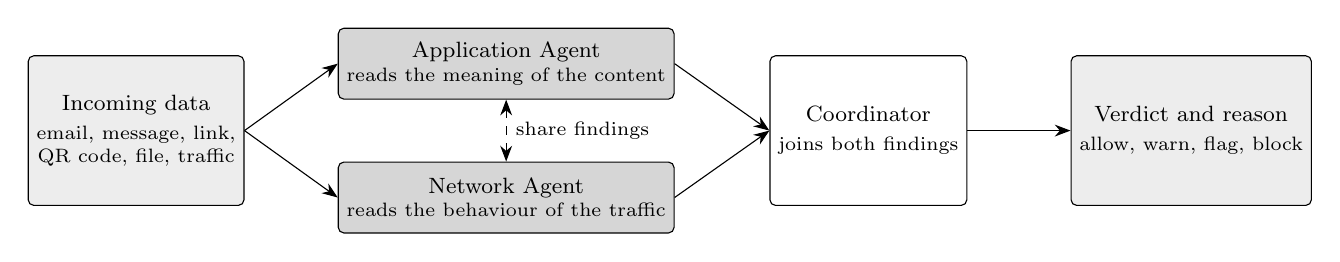
\begin{tikzpicture}[x=1cm,y=1cm]
  \node[gbox, minimum width=2.7cm, minimum height=19mm] (in) at (0,0) {Incoming data\\[1pt]{\scriptsize email, message, link,}\\[-1pt]{\scriptsize QR code, file, traffic}};
  \node[hbox, minimum width=4.1cm] (app) at (4.7,0.85) {Application Agent\\[-1pt]{\scriptsize reads the meaning of the content}};
  \node[hbox, minimum width=4.1cm] (net) at (4.7,-0.85) {Network Agent\\[-1pt]{\scriptsize reads the behaviour of the traffic}};
  \node[box, minimum width=2.5cm, minimum height=19mm] (co) at (9.3,0) {Coordinator\\[1pt]{\scriptsize joins both findings}};
  \node[gbox, minimum width=3cm, minimum height=19mm] (out) at (13.4,0) {Verdict and reason\\[1pt]{\scriptsize allow, warn, flag, block}};
  \draw[->] (in.east) -- (app.west);
  \draw[->] (in.east) -- (net.west);
  \draw[->] (app.east) -- (co.west);
  \draw[->] (net.east) -- (co.west);
  \draw[<->, dashed] (app.south) -- node[right, font=\scriptsize] {share findings} (net.north);
  \draw[->] (co) -- (out);
\end{tikzpicture}
\end{center}

\textbf{Example 1.} Someone emails the Rector of NUTECH and uses a racial slur against the Rector. The email has no virus and its traffic looks normal, so a firewall or a virus scanner sees nothing wrong. Our Application Agent understands that this is a racist insult aimed at a person, and flags it on the application layer.

\textbf{Example 2.} A polite, well-written email comes from a machine that is behaving like part of a botnet. The content looks fine, but the Network Agent raises the flag. Running both agents together is how we want to catch both cases.

\head{2. Why this is needed}
Most defences today work at one layer and depend on signatures or fixed rules. Fraud and abuse now depend on meaning. A threat can use no bad word at all, a scam can be polite, and a message can be reworded or written in Urdu or Roman Urdu to get past a keyword list. Encryption also hides the content from the network. We want one layer that joins what the application sees with what the network sees, and gives one verdict the user can trust.

\head{3. What the prototype will include}
\begin{tabularx}{\linewidth}{@{}P{3cm}YP{5.6cm}@{}}
\toprule
\textbf{Part} & \textbf{What it will do} & \textbf{How} \\
\midrule
Application Agent & Flag threats, hate and abuse, fraud and phishing. Check links and QR destinations. & Transformer models trained on public real data, with a small local language model for unclear cases and for writing the reason. \\
Network Agent & Flag attack and botnet-like behaviour from traffic metadata. & A deep model trained on real traffic captures. \\
Coordinator & Run both agents together, join their results and give one verdict. & A signed verdict record that the agents share. \\
Test gateway & Pass real email (SMTP) and web (HTTP) sessions through the layer. & Runs on our lab machines only. \\
Interfaces & Let a user check an item, and show flagged items, reasons and system health to an administrator. & A web interface first, then an Android app. \\
\bottomrule
\end{tabularx}

\newpage
\head{4. Data and testing}
We want results that are close to real use, so we will use real public data:

\begin{itemize}
  \item \textbf{Content:} public real email, SMS and online comment datasets that cover phishing, scams, threats, hate and normal messages.
  \item \textbf{Links:} live phishing feeds, with real normal web addresses from Common Crawl and the Tranco list. Live phishing links are used as text only and are never opened.
  \item \textbf{Traffic:} real captures, namely CTU-13 botnet traffic, the corrected CICIDS2017 and MAWI backbone traffic.
  \item \textbf{Our own test set:} fake fraudulent QR codes and links on reserved test domains such as \texttt{.test}, which cannot reach any real website, plus a small set of threat and abuse messages, including Urdu and Roman Urdu.
\end{itemize}

We will train on some sources and test on different ones, so the results show how the system handles data it has never seen. We will report precision, recall, F1 score, false alarm rate and time per decision. We will compare the Application Agent alone, the Network Agent alone, and both together. We will also report what fails.

\head{5. What stays out of the prototype}
The proposal describes an Internet-scale system. For the prototype we will leave out iOS, P4 and DPDK hardware paths, a real 5G core, deployment with real operators and post-quantum cryptography. Federated learning and sharing between operators will be shown on simulated operators if time allows. All of these stay in the long-term design.

\head{6. What we will deliver}
\begin{enumerate}
  \item A working prototype with its source code.
  \item A literature review of related research and published papers.
  \item A list of existing GitHub projects, showing how close each one is to our work.
  \item A research paper based on our own results, which we aim to publish.
\end{enumerate}

\head{7. How we will divide the work}
One member will lead the Application Agent and its data. One will lead the Network Agent and traffic testing. One will lead the Coordinator, the test gateway and the interfaces. All three of us will work on the evaluation and the paper.

\head{8. What I need from you}
Sir, please review this plan and tell me if you agree with the scope, or if anything should change. Once you agree, we will start implementation.

\vspace{5pt}
Regards,\\
Muhammad Abdul Ghani Qureshi

\end{document}
